
%\documentclass[aps,showpacs,amsmath,amssymb]{revtex4}
\documentclass[11pt]{article}
\usepackage{amsmath,amssymb}
\usepackage{graphics,epsfig}
\usepackage{graphicx}
\usepackage{color}
\usepackage{bm}
\usepackage{algorithmic}

\oddsidemargin=-0.0in
\evensidemargin=-0.0in
\topmargin=-0.35in
\textheight 8.9in
\textwidth 6.3in

\def\bea{\begin{eqnarray}}
\def\eea{\end{eqnarray}}
\def\be{\begin{equation}}
\def\ee{\end{equation}}
\newcommand{\bh}{{\bm h}}
\newcommand{\bk}{{\bf k}}
\newcommand{\br}{{\bf r}}
\newcommand{\bx}{{\bf x}}
\newcommand{\bt}{{\bf t}}
\newcommand{\bu}{{\bm u}}
\newcommand{\bff}{{\bm f}}
\newcommand{\bog}{{\bm \omega}}
\newcommand{\td}{\widetilde}
\newcommand{\ptl}{\partial}
\newcommand{\lal}{\langle}
\newcommand{\ral}{\rangle}
\newcommand{\lla}{\left\langle}
\newcommand{\rra}{\right\rangle}
\newcommand{\wh}{\widehat}
\newcommand{\ve}{\varepsilon}
\newcommand{\ovl}{\overline}
\newcommand{\udl}{\underline}

\begin{document}

\begin{center}
{\bf \Large \textcolor{blue}{ The JHU Turbulence Database Cluster}}
 \end{center}
 \vskip 1cm
\subsection*{DOCUMENTATION OF DATABASE FUNCTIONS}

\vskip 0.5cm
\section{Spatial differentiation inside database: equidistant grid}

In this section, $f$ denotes any one of the three components of
velocity, magnetic field, or vector potential in the $x$, $y$ and $z$ directions ($u_x$, $u_y$ or $u_z$; $b_x$, $b_y$ or $b_z$; $a_x$, $a_y$ or $a_z$), or pressure ($p$), depending on which function is called. $\Delta x$ and $\Delta y$ are the width of grid in $x$ and $y$ direction.

\subsection{Options for GetVelocityGradient, GetMagneticFieldGradient, GetVectorPotentialGradient, and GetPressureGradient}

\begin{figure}[h]
\begin{minipage}{\linewidth}
\centering\includegraphics[width=1.0\linewidth]{1DGrid.eps}
\end{minipage} \caption{Illustration of data points along x direction. The same approach is used in the y and z directions.}\label{1DGrid}
\end{figure}

\subsubsection*{FD4: 4th-order centered finite differencing}
\label{sec-FD4}

With the edge replication of 4 data-points on each side, this option can be spatially interpolated using 4th-order Lagrange Polynomial interpolation.

\bea \left.\frac{df}{dx}\right|_{x_n}
&=& \frac{2}{3\Delta x}[f(x_{n+1})-f(x_{n-1})]-\frac{1}{12\Delta
x}[f(x_{n+2})-f(x_{n-2})]\nonumber\\
&&+o(\Delta x^4) \eea

\subsubsection*{FD6: 6th-order centered finite differencing}

\bea \left.\frac{df}{dx}\right|_{x_n} &=&
\frac{3}{4\Delta
x}[f(x_{n+1})-f(x_{n-1})]-\frac{3}{20\Delta x}[f(x_{n+2})-f(x_{n-2})]\nonumber\\
&&+\frac{1}{60\Delta x}[f(x_{n+3})-f(x_{n-3})]+o(\Delta x^6) \eea

\subsubsection*{FD8: 8th-order centered finite differencing}
With the edge replication of 4 data-points on each side, this is the highest-order finite difference option available.
\bea \left.\frac{df}{dx}\right|_{x_n} &=&
\frac{4}{5\Delta
x}[f(x_{n+1})-f(x_{n-1})]-\frac{1}{5\Delta x}[f(x_{n+2})-f(x_{n-2})]\nonumber\\
&&+\frac{4}{105\Delta x}[f(x_{n+3})-f(x_{n-3})]-\frac{1}{280\Delta
x}[f(x_{n+4})-f(x_{n-4})]\nonumber\\
&& +o(\Delta x^8) \eea

\subsection{Options for GetVelocityLaplacian, GetMagneticFieldLaplacian, GetVectorPotentialLaplacian, GetVelocityHessian, GetMagneticFieldHessian, GetVectorPotentialHessian, and
GetPressureHessian}
In this section, second derivatives finite difference evaluations are shown. The expressions are
given for derivatives along single directions in terms of the x-direction, and mixed derivatives are
illustrated on the x-y plane. The same approach is used in the y and z directions, as well as in the x-z and y-z planes
for the other mixed derivatives.
 \begin{figure}[h]
\begin{minipage}{\linewidth}
\centering\includegraphics[width=1.0\linewidth]{2DGrid.eps}
\end{minipage} \caption{Illustration of data points on $x-y$ plane. The same approach is used in the $x-z$ and $y-z$ planes.}\label{2DGrid}
\end{figure}

\subsubsection*{FD4: 4th-order centered finite differencing (can be spatially
interpolated using 4th-order Lagrange Polynomial interpolation}
\bea \left.\frac{d^2f}{dx^2}\right|_{(x_m,y_n)} &=&
\frac{4}{3\Delta
x^2}[f(x_{m+1},y_n)+f(x_{m-1},y_n)-2f(x_m,y_n)]\nonumber\\
&&-\frac{1}{12\Delta
x^2}[f(x_{m+2},y_n)+f(x_{m-2},y_n)-2f(x_m,y_n)]\nonumber\\
&&+o(\Delta x^4) \eea

\bea \left.\frac{d^2f}{dxdy}\right|_{(x_m,y_n)} &=&
\frac{1}{3\Delta
x\Delta y}[f(x_{m+1},y_{n+1})+f(x_{m-1},y_{n-1})\nonumber\\
&&-f(x_{m+1},y_{n-1})-f(x_{m-1},y_{n+1})]\nonumber\\
&&-\frac{1}{48\Delta
x\Delta y}[f(x_{m+2},y_{n+2})+f(x_{m-2},y_{n-2})\nonumber\\
&&-f(x_{m+2},y_{n-2})-f(x_{m-2},y_{n+2})]\nonumber\\
&&+o(\Delta x^4) \eea

\subsubsection*{FD6: 6th-order centered finite differencing}
\bea \left.\frac{d^2f}{dx^2}\right|_{(x_m,y_n)}
&=& \frac{3}{2\Delta
x^2}[f(x_{m+1},y_n)+f(x_{m-1},y_n)-2f(x_m,y_n)]\nonumber\\
&&-\frac{3}{20\Delta
x^2}[f(x_{m+2},y_n)+f(x_{m-2},y_n)-2f(x_m,y_n)]\nonumber\\
&&+\frac{1}{90\Delta
x^2}[f(x_{m+3},y_n)+f(x_{m-3},y_n)-2f(x_m,y_n)]\nonumber\\
&&+o(\Delta x^6) \eea

\bea \left.\frac{d^2f}{dxdy}\right|_{(x_m,y_n)} &=&
\frac{3}{8\Delta
x\Delta y}[f(x_{m+1},y_{n+1})+f(x_{m-1},y_{n-1})\nonumber\\
&&-f(x_{m+1},y_{n-1})-f(x_{m-1},y_{n+1})]\nonumber\\
&&-\frac{3}{80\Delta
x\Delta y}[f(x_{m+2},y_{n+2})+f(x_{m-2},y_{n-2})\nonumber\\
&&-f(x_{m+2},y_{n-2})-f(x_{m-2},y_{n+2})]\nonumber\\
&&+\frac{1}{360\Delta
x\Delta y}[f(x_{m+3},y_{n+3})+f(x_{m-3},y_{n-3})\nonumber\\
&&-f(x_{m+3},y_{n-3})-f(x_{m-3},y_{n+3})]\nonumber\\
&&+o(\Delta x^6) \eea

\subsubsection*{FD8: 8th-order centered finite differencing}
\bea \left.\frac{d^2f}{dx^2}\right|_{(x_m,y_n)}
&=& \frac{792}{591\Delta
x^2}[f(x_{m+1},y_n)+f(x_{m-1},y_n)-2f(x_m,y_n)]\nonumber\\
&&-\frac{207}{2955\Delta
x^2}[f(x_{m+2},y_n)+f(x_{m-2},y_n)-2f(x_m,y_n)]\nonumber\\
&&-\frac{104}{8865\Delta
x^2}[f(x_{m+3},y_n)+f(x_{m-3},y_n)-2f(x_m,y_n)]\nonumber\\
&&+\frac{9}{3152\Delta
x^2}[f(x_{m+4},y_n)+f(x_{m-4},y_n)-2f(x_m,y_n)]\nonumber\\
&&+o(\Delta x^8) \eea

\bea \left.\frac{d^2f}{dxdy}\right|_{(x_m,y_n)} &=&
\frac{14}{35\Delta
x\Delta y}[f(x_{m+1},y_{n+1})+f(x_{m-1},y_{n-1})\nonumber\\
&&-f(x_{m+1},y_{n-1})-f(x_{m-1},y_{n+1})]\nonumber\\
&&-\frac{1}{20\Delta
x\Delta y}[f(x_{m+2},y_{n+2})+f(x_{m-2},y_{n-2})\nonumber\\
&&-f(x_{m+2},y_{n-2})-f(x_{m-2},y_{n+2})]\nonumber\\
&&+\frac{2}{315\Delta
x\Delta y}[f(x_{m+3},y_{n+3})+f(x_{m-3},y_{n-3})\nonumber\\
&&-f(x_{m+3},y_{n-3})-f(x_{m-3},y_{n+3})]\nonumber\\
&&-\frac{1}{2240\Delta
x\Delta y}[f(x_{m+4},y_{n+4})+f(x_{m-4},y_{n-4})\nonumber\\
&&-f(x_{m+4},y_{n-4})-f(x_{m-4},y_{n+4})]\nonumber\\
&&+o(\Delta x^8) \eea

\section{Spatial interpolation inside database: equidistant grid}
\label{sec:spa}
\begin{figure}[h]
\begin{minipage}{\linewidth}
\centering\includegraphics[width=1.0\linewidth]{Lagrangian.eps}
\end{minipage} \caption{Illustration of Lagrangian interpolation. }\label{Lagrangian}
\end{figure}
\subsection{Interpolation Options for GetVelocity, GetMagneticField, GetVectorPotential, GetPressure and GetVelocityAndPressure}
In this section, $f$ denotes any one of the three components of
velocity, $u_x$, $u_y$ or $u_z$, magnetic field $b_x$, $b_y$ or $b_z$, vector potential $a_x$, $a_y$ or $a_z$, or pressure, $p$,  depending on which
function is called. $\Delta x$, $\Delta y$ and $\Delta z$ are the
width of grid in $x$, $y$ and $z$ direction. ${\bf x'}=(x',y',z')$.
\subsubsection*{NoSInt: No spatial  interpolation}
\label{sec-noint}
In this case, the value at the datapoint closest to each
coordinate value is returned, rounding up or down in each
direction. \bea f({\bf x'}) &=& f(x_n,y_p,z_q)\eea where
$n=int(\frac{x'}{\Delta x}+\frac{1}{2})$, $p=int(\frac{y'}{\Delta
y}+\frac{1}{2})$, $q=int(\frac{z'}{\Delta z}+\frac{1}{2})$.

\subsubsection*{Lag4: 4th-order Lagrange Polynomial interpolation}

In this case, 4th-order Lagrange Polynomial interpolation is done along each spatial direction.
\bea f({\bf x'}) &=&
\sum_{i=1}^4\sum_{j=1}^4\sum_{k=1}^4f(x_{n-2+i},y_{p-2+j},z_{q-2+k})\nonumber\\
&&\cdot l_x^{n-2+i}(x')\cdot l_y^{p-2+j}(y')\cdot
l_z^{q-2+k}(z')\eea \bea l_\theta^i(\theta') &=&
\frac{\prod\limits_{j=n-1,j\neq
i}^{n+2}(\theta'-\theta_j)}{\prod\limits_{j=n-1,j\neq
i}^{n+2}(\theta_i-\theta_j)}\eea where $\theta$ can be x, y, or z.

\subsubsection*{Lag6: 6th-order Lagrange Polynomial interpolation}

In this case, 6th-order Lagrange Polynomial interpolation is done along each spatial direction.
\bea f({\bf x'}) &=&
\sum_{i=1}^6\sum_{j=1}^6\sum_{k=1}^6f(x_{n-3+i},y_{p-3+j},z_{q-3+k})\nonumber\\
&&\cdot l_x^{n-3+i}(x')\cdot l_y^{p-3+j}(y')\cdot
l_z^{q-3+k}(z')\eea \bea l_\theta^i(\theta') &=&
\frac{\prod\limits_{j=n-2,j\neq
i}^{n+3}(\theta'-\theta_j)}{\prod\limits_{j=n-2,j\neq
i}^{n+3}(\theta_i-\theta_j)}\eea where $\theta$ can be x, y, or z.

\subsubsection*{Lag8: 8th-order Lagrange Polynomial interpolation}

In this case, 8th-order Lagrange Polynomial interpolation is done along each spatial direction.
\bea f({\bf x'}) &=&
\sum_{i=1}^8\sum_{j=1}^8\sum_{k=1}^8f(x_{n-4+i},y_{p-4+j},z_{q-4+k})\nonumber\\
&&\cdot l_x^{n-4+i}(x')\cdot l_y^{p-4+j}(y')\cdot
l_z^{q-4+k}(z')\eea \bea l_\theta^i(\theta') &=&
\frac{\prod\limits_{j=n-3,j\neq
i}^{n+4}(\theta'-\theta_j)}{\prod\limits_{j=n-3,j\neq
i}^{n+4}(\theta_i-\theta_j)}\eea where $\theta$ can be x, y, or z.

\subsection{Interpolation Options for GetVelocityGradient, GetVelocityLaplacian, GetVelocityHessian, GetMagneticFieldGradient, GetVectorPotentialGradient,
 GetMagneticFieldLaplacian, GetVectorPotentialLaplacian, GetMagneticFieldHessian, GetVectorPotentialHessian, GetPressureGradient, and GetPressureHessian}

In this section, $f$ denotes gradients of velocity, magnetic field, vector potential, or pressure gradient,
Laplacian of velocity, magnetic field, vector potential, or Hessian of velocity, magnetic field, vector potential or pressure, depending on
which function is called.
\subsubsection*{FD4NoInt, FD6NoInt and FD8NoInt: No spatial  interpolation}

In this case, the value of the 4th, 6th, or 8th order finite-difference
evaluation of the derivative at the datapoint closest to each coordinate value is
returned, rounding up or down in each direction.
\bea f({\bf x'}) &=& f(x_n,y_p,z_q)\eea where
$n=int(\frac{x'}{\Delta x}+\frac{1}{2})$, $p=int(\frac{y'}{\Delta
y}+\frac{1}{2})$, $q=int(\frac{z'}{\Delta z}+\frac{1}{2})$.

\subsubsection*{FD4Lag4: 4th-order Lagrange Polynomial interpolation of 4th-order finite diff.}

In this case, the values of the 4th order finite-difference
evaluation of the derivative at the data points are interpolated using 4th-order Lagrange Polynomials.
\bea f({\bf x'}) &=&
\sum_{i=1}^4\sum_{j=1}^4\sum_{k=1}^4f(x_{n-2+i},y_{p-2+j},z_{q-2+k})\nonumber\\
&&\cdot l_x^{n-2+i}(x')\cdot l_y^{p-2+j}(y')\cdot
l_z^{q-2+k}(z')\eea \bea l_\theta^i(\theta') &=&
\frac{\prod\limits_{j=n-1,j\neq
i}^{n+2}(\theta'-\theta_j)}{\prod\limits_{j=n-1,j\neq
i}^{n+2}(\theta_i-\theta_j)}\eea where $\theta$ can be x, y, or z.

\section{Spatial interpolation inside the database: non-uniform grid}\label{sec:interp}
Spatial interpolation for domains with non-uninform grid spacing (e.g. the
channel flow domain) is applied using multivariate polynomial interpolation of
the barycentric Lagrange form from Ref.~\cite{Berrut2004}. Using this approach,
we are interested in interpolating the field $f$ at point $\bm{x}^\prime$. The
point $\bm{x}^\prime$ is known to exist within the grid cell at location
$(x_m,y_n,z_p)$ where $(m,n,p)$ are the cell indices. The cell indices are
obtained for the $x$ and $z$ directions, which are uniformly distributed,
according to
\begin{align}
  m &= \text{floor}( x^\prime / dx ) \\
  p &= \text{floor}( z^\prime / dz ) \mbox{ .} \notag
\end{align}
In the $y$ direction the grid is formed by Marsden-Schoenberg collocation points
which are not uniformly distributed. Along this direction we perform a search to obtain $n$ such that 
\begin{align}
  y_n  \leq y^\prime < y_{n+1} &\text{\hspace{1ex} if } y^\prime \leq 0 \\
  y_{n-1} < y^\prime \leq y_n &\text{\hspace{1ex} if } y^\prime > 0 \notag
\end{align}

The cell indices are also assured to obey the following:
\begin{align}
  0 \leq m \leq N_x - 2 & \notag \\
  0 \leq n \leq N_y/2 - 1 &\text{\hspace{1ex} if } y^\prime \leq 0 \\
  N_y/2 \leq n \leq N_y - 1 &\text{\hspace{1ex} if } y^\prime > 0 \notag \\
  0 \leq p \leq N_z - 2 &\notag
\end{align}
where $N_x$, $N_y$, and $N_z$ are the number of grid points along the $x$, $y$, and
$z$ directions, respectively. In the case that $x^\prime = x_{N_x-1}$ the cell index set to be $m=N_x-2$; likewise for the $z$ direction.
 
The interpolation stencil also contains $q$ points in each direction for an order $q$
interpolant (with degree $q-1$). The resulting interpolated value is expressed as:
\begin{equation}\label{eq:interp_poly}
  f(\bm{x}^\prime) = \sum_{i=i_s}^{i_e}\sum_{j=j_s}^{j_e}\sum_{k=k_s}^{k_e}  l_x^{i}(x^\prime) l_y^{j}(y^\prime) l_z^{k}(z^\prime)f(x_{i}, y_{j}, z_{k})
\end{equation}
where the starting and ending indices are given as
\begin{align}
i_s &= m - \text{ceil}(q/2) + 1\notag\\
i_e &= i_s + q - 1 \notag\\
j_s &= 
\begin{cases} 
  n - \text{ceil}(q/2) + 1 + j_o &\mbox{if } n \leq N_y / 2 - 1 \\
  n - \text{floor}(q/2) + j_o &\mbox{otherwise} 
\end{cases} \\
j_e &= j_s + q - 1 \notag\\
k_s &= p - \text{ceil}(q/2) + 1 \notag\\
k_e &= k_s + q - 1 \notag
\end{align}
and $j_o$ is the index offset for the $y$ direction depending on the distance from the top and bottom walls. The $\text{ceil}()$ function ensures that stencil remains symmetric about the interpolation point when $q$ is odd. In the case for $j_s$, the separate treatments for the top and bottom halves of the channel is done to ensure that the one-sided stencils remain symmetric with respect to the channel center. The value for $j_o$ may be evaluated based upon the $y$ cell index and the interpolation order as 
\begin{equation}
  j_o = 
  \begin{cases} 
    \text{max}(\text{ceil}(q/2)-n-1,0) &\mbox{if } n \leq N_y/2-1 \\
    \text{min}(N_y - n - \text{ceil}(q/2),0) & \mbox{otherwise}  
  \end{cases}	
  \mbox{ .}
\end{equation}

The interpolation weights, $l_x$, $l_y$, and $l_z$, are given as
\begin{equation}\label{eq:interp_poly_coefs}
  l_\theta^\xi(\theta^\prime) = \frac{\frac{w_\xi}{\theta^\prime - \theta_\xi}}{\sum_{\eta=\xi_s}^{\xi_e} \frac{w_{\eta}}{\theta^\prime - \theta_\eta} }
\end{equation}
where $\theta$ may either be $x$, $y$, or $z$. The barycentric weights, $w_\xi$, in \eqref{eq:interp_poly_coefs} are given as
\begin{equation}\label{eq:interp_bary_weight}
  w_\xi = \frac{1}{\prod_{\eta=\xi_s,\eta\neq \xi}^{\xi_e} \theta_\xi - \theta_\eta}
\end{equation}
The weights are computed by applying a recursive update procedure as in Ref.\cite{Berrut2004}. A slightly modified version of the algorithm in Ref.~\cite{Berrut2004} is given below:
\begin{algorithmic}
  \FOR{$\xi=\xi_s$ to $\xi_e$}\STATE{$w_\xi = 1$}\ENDFOR
  \FOR {$\xi = \xi_s +1$ to $\xi_e$}  
  \FOR {$\eta = \xi_s$ to $\xi-1$} 
  \STATE{
    $w_\eta = (\theta_\eta - \theta_\xi) w_\eta$ \\
    $w_\xi = (\theta_\xi - \theta_\eta) w_\xi$ 
  }
  \ENDFOR
  \ENDFOR
  \FOR{$\xi=\xi_s$ to $\xi_e$}\STATE{$w_\xi = 1/w_\xi$}\ENDFOR
\end{algorithmic}

To account for the periodic domain along the $x$ and $z$ directions we adjust the $i$ and $k$ indices when referencing $f$ in \eqref{eq:interp_poly} such that
\begin{equation}
  f(\bm{x}^\prime) = \sum_{i=i_s}^{i_e}\sum_{j=j_s}^{j_e}\sum_{k=k_s}^{k_e}  l_x^{i}(x^\prime) l_y^{j}(y^\prime) l_z^{k}(z^\prime)f(x_{i\%Nx}, y_{j}, z_{k\%Nz})
\end{equation}
and $\%$ is the modulus operator. The indices for the interpolation coefficients remain the same, however, we use the fact that the grid points are uniformly spaced such that \eqref{eq:interp_poly_coefs} becomes
\begin{equation}
  l_\theta^\xi(\theta^\prime) = \frac{\frac{w_\xi}{\theta^\prime - \xi \Delta\theta}}{\sum_{\eta=\xi_s}^{\xi_e} \frac{w_{\eta}}{\theta^\prime - \eta \Delta\theta} }
\end{equation}
and similarly for the barycentric weights, \eqref{eq:interp_bary_weight} becomes
\begin{equation}\label{eq:interp_bary_weight_periodic}
  w_\xi = \frac{1}{\prod_{\eta=\xi_s,\eta\neq \xi}^{\xi_e} (\xi - \eta)\Delta\theta}
\end{equation}
for the $x$ and $z$ directions. The computation of the barycentric weights for the $x$ and $z$ directions are carried out once (for a given interpolation order) for all grid points using \eqref{eq:interp_bary_weight_periodic}; for the $y$ direction the barycentric weights are computed for each point using \eqref{eq:interp_bary_weight}.

\section{Spatial differentiation inside the database: non-uniform grid}
Spatial differentiation for grids with non-uniform spacing is performed using the barycentric method of the interpolating polynomial. In one dimension (assuming the $x$ direction; the same applies for the $y$ and $z$ directions), the interpolant for the field $f$ is given as
\begin{equation}
f(x) = \sum_{j=i_s}^{i_e} l^{j}_x(x) f(x_j) \text{ .}
\end{equation}
It follows that the $r^{th}$ derivative may be computed as
\begin{equation}
\frac{d^rf}{dx^r}(x) = \sum_{j=i_s}^{i_e} \frac{d^r l^{j}_x}{dx^r}(x) f(x_j) \text{ .}
\end{equation}
Within the database we compute the derivatives at the grid sites for the $FD4NoInt$, $FD6NoInt$, and $FD8NoInt$ differencing methods where no interpolation is performed. If a sample point is given that does not coincide with a grid point, the derivative at the \textit{nearest} grid point is computed and returned. For the $FD4Lag4$ method we compute the derivatives with the $FD4NoInt$ method (at the grid sites) and then these data are interpolated to the interpolation point using the $Lag4$ interpolation method presented in \S\ref{sec:interp}. 

For evaluating derivatives at the grid sites we follow the method presented in Ref.~\cite{Berrut2004} such that
\begin{equation}
\frac{d^rf}{dx^r}(x_i) = \sum_{j=i_s}^{i_e} D^{(r)}_{x,ij} f(x_j) \text{ .}
\end{equation}
where $D^{(r)}_{x,ij} = \frac{d^r l^{j}_x}{dx^r}(x_i)$ is the differentiation matrix~\cite{Berrut2004}. The differentiation matrices for $r=1$ and $r=2$ are given, respectively, as
\begin{align}
D^{(1)}_{x,ij} &= \frac{w_j / w_i}{x_i - x_j} \\\label{eq:l_second_deriv}
D^{(2)}_{x,ij} &= -2\frac{w_j / w_i}{x_i - x_j}\left[\sum_{k \neq i} \frac{w_k / w_i}{x_i - x_k} + \frac{1}{x_i-x_j}\right]
\end{align}
for $i \neq j$ and
\begin{equation}\label{eq:l_i_eq_j}
D^{(r)}_{x,jj} = -\sum_{i\neq j} D^{(r)}_{x,ji}
\end{equation}
when $i = j$ for all $r>0$. We note that in \eqref{eq:l_second_deriv} and \eqref{eq:l_i_eq_j} fixes have been applied to the respective equations presented in Ref.~\cite{Berrut2004}, i.e., (9.4) and (9.5). As with the interpolation schemes, the grid point locations for the uniformly distributed directions are expressed as $\theta_\xi = \xi \Delta\theta$, where $\theta$ may either be $x$ or $z$. 

For second order mixed derivatives (such as for the pressure Hessian) we compute the derivatives at the grid sites within the respective plane. When computing the mixed partials along $x$ and $y$ we have
\begin{equation}
\frac{d^2f}{dxy}(x_m,y_n) = \sum_{i=i_s}^{i_e} \sum_{j=j_s}^{j_e} D^{(1)}_{x,mi} D^{(1)}_{y,nj} f(x_i,y_j) \textbf{ .}
\end{equation}
Similar formulae exist for mixed partials along $x$ and $z$, and $y$ and $z$. 

The differencing stencil size depends on the required order of the differencing method and the derivative order, $r$. In general, the resulting stencil size is determined as
\begin{equation}
q = 
\begin{cases}
  q^\prime + r & \text{ for non--symmetric grid distribution about evaluation point} \\
  q^\prime +r-(r+1)\%2 & \text{ for symmetric grid distribution about evalutation point} 
\end{cases}
\end{equation}
where $q^\prime$ is the order of the differencing method. For example, to obtain a $6^{th}$ order differencing method for the first derivative of $f$ along the $x$, $y$, and $z$ directions, a value of $q=7$ is required. For the second derivative, the $x$ or $z$ directions require a value of $q=7$ where the $y$ direction requires $q=8$ to acheive a $6^{th}$ order differencing method.

\section{Temporal interpolation inside database}
\label{sec:tem}
\begin{figure}[h]
\begin{minipage}{\linewidth}
\centering\includegraphics[width=0.5\linewidth]{PCHIP.eps}
\end{minipage} \caption{Illustration of data points for time.}\label{PCHIP}
\end{figure}

In this section, $f$ denotes velocity, magnetic field, vector potential, pressure,
their gradient, Laplacian or Hessian, or force, depending on which function is called. $\Delta t$ is
the time increment between consecutive times stored in the database.

\subsection*{NoTInt: No temporal interpolation}

In this case, the value at the datapoint closest to the time value
is returned, rounding up or down. \bea f(t') &=& f(t_n)\eea where
$n=int(\frac{t'}{\Delta t}+\frac{1}{2})$.

\subsection*{PCHIP: Cubic Hermite Interpolation in time}

The value from the two nearest time points is interpolated at time $t'$
using Cubic Hermite Interpolation Polynomial, with centered finite
difference evaluation of the end-point time derivatives - i.e. a
total of four temporal points are used. \bea
f(t')=a+b(t'-t_n)+c(t'-t_n)^2+d(t'-t_n)^2(t'-t_{n+1}) \eea where
\bea a &=& f(t_n)\nonumber\eea \bea b &=&
\frac{f(t_{n+1})-f(t_{n-1})}{2\Delta t}\nonumber\eea \bea c &=&
\frac{f(t_{n+1})-2f(t_n)+f(t_{n-1})}{2\Delta t^2}\nonumber\eea
\bea d &=&
\frac{-f(t_{n-1})+3f(t_n)-3f(t_{n+1})+f(t_{n+2})}{2\Delta t^3}
\nonumber\eea

\section{Spatial filtering inside database} 

\begin{figure}[ht]
\begin{minipage}{\linewidth}
\centering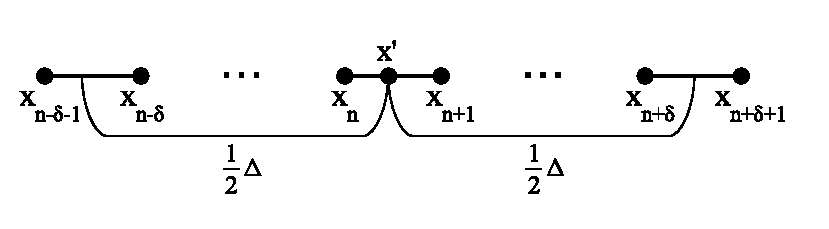
\includegraphics[width=0.8\linewidth]{Filtering.eps}
\end{minipage} \caption{Illustration of data points for filtering.}\label{filtering}
\end{figure}

In this section, $f$ denotes any one of the three components of velocity, $u_x$, $u_y$ or $u_z$, 
magnetic field $b_x$, $b_y$ or $b_z$, vector potential $a_x$, $a_y$ or $a_z$, or pressure, $p$,  
depending on the user supplied parameter for the GetBoxFilter and GetBoxFilterGradient functions called $field$. If the 
GetBoxFilterSGS function is called, $f$ denotes any one of the six components of the sub-grid
stress tensor for the respective field (e.g. $u_x^2$, $u_y^2$, $u_z^2$, $u_x u_y$, $u_x u_z$, $u_y u_z$).
The valid values
for the $field$ parameter are $velocity, magnetic, potential, pressure$. $\Delta x$ is the resolution of the grid
(it is equal in all directions). The user also supplies the desired 
filter width $\Delta$, which is given as a floating point number and is required to be an odd multiple of the grid
resolution (to eliminate the need for interpolating at the edges). ${\bf x'}=(x',y',z')$. 

\subsection{GetBoxFilter and GetBoxFilterSGS}
The box filter around the target location and with the given filter width is computed as follows:
\bea \overline{f({\bf x'})} &=& \frac{1}{\Delta^3} \cdot
\sum_{i=n - \delta}^{n + \delta}\sum_{j=p - \delta}^{p + \delta}\sum_{k=q - \delta}^{q + \delta}f(x_{i},y_{j},z_{k}),\eea
where $n=int(\frac{x'}{\Delta x}+\frac{1}{2})$, $p=int(\frac{y'}{\Delta
y}+\frac{1}{2})$, $q=int(\frac{z'}{\Delta z}+\frac{1}{2})$, and $\delta = int(\frac{1}{2}\frac{\Delta}{\Delta x}$).

\subsection{GetBoxFilterGradient}
In this case, the computation of the gradient is done by means of second order finite differencing of the filtered values. 
In addition to the $field$ and $filter$ $width$ parameters described above the user can request a particular spacing for 
the finite differencing computation, $\Delta x'$. The filtered values computed as above are used to compute the filtered
value of the gradient according to:
\bea \left.\overline{\frac{df}{dx}}\right|_{x_n}
&=& \frac{1}{2\Delta x'}[\overline{f(x_{n+h})}-\overline{f(x_{n-h})}] +o({\Delta x'}^2), \eea
where $h = int(\frac{\Delta x'}{\Delta x}$).

\section{Evaluating the applied force inside database using GetForce for hydrodynamic isotropic turbulence dataset (``isotropic1024'')}

Information about the forcing term $f_i(x,y,z,t)$ (force per unit mass, $i=x,y,z$) applied during the DNS has been stored inside the database and can be retrieved using the function GetForce. During DNS, an effective forcing is applied in Fourier space by rescaling low-k Fourier modes (with magnitudes $0.5\leq k\leq 2.5$, $k=\sqrt{k_x^2+k_y^2+k_z^2}$) to maintain their kinetic energy to prescribed values consistent with a $-5/3$ spectrum. The forcing region is divided into two shells,
$0.5\leq k\leq 1.5$ and $1.5<k\leq 2.5$, and the spectrum is fixed at a value of $0.3$ in shell $0.5\leq k\leq 1.5$ shell and 0.13 in shell $1.5<k\leq 2.5$ shell (these values are obtained empirically so that the simulated spectrum is close to $k^{-5/3}$ at low $k$).

In order to represent the rescaling in terms of a forcing term, we interpreting the time-advancement in terms of a
first-order time-advancement and write the discretized Navier-Stokes equation (NSE) in Fourier space as follows
\bea
\hat{u}_i^{n+1}(k_x,k_y,k_z) = \hat{u}_i^{n+}(k_x,k_y,k_z)+\hat{f}_i(k_x,k_y,k_z) dt
\label{eq:ui^{n+1}}
\eea
in which $\hat{u}_i^{n+}=\hat{u}_i^n+(\cdots)dt$ with $(\cdots)$ for terms on the right-hand side of NSE excluding the forcing term, and $dt$ is the time-step of the DNS.

In the DNS, the rescaling induces a difference between $\hat{u}_i^{n+}$ and $\hat{u}_i^{n}$ in the wave-number range $0.5\leq k\leq 2.5$  that is equivalent to a force-term
defined in the two shells as follows
\bea
 \hat {f}^n_i(k_x,k_y,k_z)=\frac{1}{dt} \left(\sqrt{\frac{0.3}{\sum_{0.5\leq k \leq 1.5}[(\hat {u}^{n+}_x)^2+(\hat {u}^{n+}_y)^2+(\hat {u}^{n+}_z)^2)]/2}}-1\right)~\hat {u}^{n+}_i(k_x,k_y,k_z)
\eea
for shell $0.5\leq k \leq 1.5$ and
\bea
 \hat {f}^n_i(k_x,k_y,k_z)=\frac{1}{dt} \left(\sqrt{\frac{0.13}{\sum_{1.5\leq k \leq 2.5}[(\hat {u}^{n+}_x)^2+(\hat {u}^{n+}_y)^2+(\hat {u}^{n+}_z)^2)]/2}}-1\right)~\hat {u}^{n+}_i(k_x,k_y,k_z)
\eea
for shell $1.5< k \leq 2.5$, where $\hat u_x$,  $\hat u_y$,  $\hat u_z$ denote the three velocity components in Fourier space and   $k=\sqrt{k_x^2+k_y^2+k_z^2}$ is the magnitude of wavenumber vector ${\bf  k}$. In this way, the energy in these shells $E(k=1)=\sum_{0.5\leq k \leq 1.5}(\hat {u}_x^2+\hat {u}_y^2+\hat {u}_z^2)/2$ and $E(k=2)=\sum_{1.5< k \leq 2.5}(\hat {u}_x^2+\hat {u}_y^2+\hat {u}_z^2)/2$ is maintained at 0.3 and 0.13.

There exist in total of 80 discrete wave-number modes in these two shells. There are 20 modes for $k_x=0$, 30 for $k_x>0$, and another 30 for $k_x<0$. In the database, the complex Fourier coefficients $\hat f_x$, $\hat f_y$, $\hat f_z$ corresponding to $k_x\geq 0$ (50 modes) are stored, the remaining 30 modes ($k_x<0$) are the conjugates of the modes $k_x>0$.

Using the GetForce function, force values at any prescribed position $(x,y,z)$ are evaluated in the database from the Fourier forcing coefficients according to direct summation of the Fourier series according to
\bea
f_i(x,y,z,t_n)= \sum_{k_x,k_y,k_z} ~e^{i(k_xx+k_yy+k_zz)}~\hat {f^n_i}(k_x,k_y,k_z)
\eea
where $i$ can be $x$, $y$, and $z$. Values of $f_i(x,y,z,t)$ at arbitrary times $t$ can be obtained by specifying PCHIP temporal interpolation.

\section{Evaluating the applied force inside database using GetForce for MHD turbulence dataset (``mhd1024'')}

Using the GetForce function, force values at any prescribed position $(x,y,z)$ are evaluated in the Taylor-Green prescribed force field according to
\bea
f_x(x,y,z,t_n)= 0.25 \sin(2x)\cos(2y)\cos(2z)
\eea
\bea
f_y(x,y,z,t_n)=  - 0.25 \cos(2x)\sin(2y)\cos(2z)
\eea
\bea
f_z(x,y,z,t_n)= 0.
\eea
 

\section{Tracking fluid particles by GetPosition function}

Getposition function  tracks arrays of particles  simultaneously and returns final particle locations at the end of the trajectory integration time. The function uses second order time Runge-Kutta integration.

Given particle locations ${\bf y}$ at a start time ($t_{ST}$), the function returns all the particle locations at a user defined end time ($t_{ET}$) with user-specified particle integration time-step ($\Delta t_p$). Forward tracking is accomplished by specifying $t_{ET}>t_{ST}$, whereas backward tracking is accomplished by specifying  $t_{ET}<t_{ST}$. The time-step $\Delta t_p$'s sign need not be specified to make the distinction between forward and backward tracking since inside the tracking integration, it is taken to be sign$[t_{ET}-t_{ST}] |\Delta t_p|$. 
   
Particle tracking is accomplished by integrating between times $t_{ST}$ and $t_{ET}$ the equation
%each particle is tagged and randomly assigned an initial position.
% Huidan - not sure what you mean by randomly assigned -- the user specifies the initial position, no?
\begin{equation}
\frac{\partial {\bf  x}^+({\bf y},t)}{\partial t}={\bf u}^+({\bf y},t)
\label{eq:particlemotionequation}
\end{equation}
where ${\bf x}^+({\bf y},t)$ and ${\bf u}^+({\bf y},t)$ denotes the position and velocity at time t of the fluid particle originating from position ${\bf y}$ at initial time $t_{ST}$ (superscript $+$ represents Lagrangian quantities following the fluid particle).  
The  Lagrangian velocity ${\bf u}^+({\bf y},t)$ is replaced by the Eulerian velocity from the database ${\bf u}({\bf x},t)$ where the particle is located, namely ${\bf u}^+({\bf y},t)={\bf u}({\bf x}^+({\bf y},t),t)$.

To advance the particle positions between two successive time instants $t_m$ and $t_{m+1}(=t_m+\Delta t_p)$   the predictor step yields an estimate
\begin{equation}
{\bf x}^*={\bf x}^+({\bf y},t_m) + \Delta t_p ~{\bf u}^+({\bf y},t_m).
\label{eq:pre_position}
\end{equation}
The corrector step then gives the particle position at $t_{m+1}$ as
\begin{equation}
{\bf x}^+({\bf y},t_{m+1})={\bf x}^+({\bf y},t_m)+\Delta t_p ~[{\bf u}^+({\bf y},t_m)+{\bf u}^+({\bf x}^*,t_{n+1})]/2.
\label{eq:position}
\end{equation}
The integration proceeds until $t_m$ reaches the user-specified final time $t_{ES}$. The last integration time-step is typically done using a smaller time-step so that the integration ends exactly at the specified $t_{ES}$. GetPosition then returns ${\bf x}^+({\bf y},t_{ES})$ for all particles that were at initial locations ${\bf y}$.

For this integration scheme, the time-stepping error is of order $(\Delta t_p)^3$ over one time step. In general, accurate spatial and time interpolations are crucial to obtain the fluid velocities while tracking particles along their trajectories. Spatial interpolation with various optional orders of accuracy can be specified by the user, see \S\ref{sec:spa}  above. Time interpolation is done by default using PHCIP (see \S\ref{sec:tem} above).

\bibliographystyle{plain}
\bibliography{Database-functions}
\end{document}
